\documentclass{swjtuthesis}

\addbibresource{example.bib}
\nocite{*}

\begin{document}

\title{Thesis' Title}
\grade{Grade}
\stunum{Student Number}
\author{Name}
\major{Major}
\instructor{Instructor}
\department{Department}
\maketitlepage

\makeais
\makecua
\makeevaluatepage

\startabstract
\keywords{关键词1;关键词2;关键词3}
\enkeywords{kw1; kw2; kw3; kw4; kw5}
\begin{abstract}
    Web信息的爆炸性增长使Internet成为我们获取信息资源的重要途径,而在全球一体化的今天,人们对翻译质量和翻译速度的要求也日趋严格。网络上拥有大量的双语对照信息,而传统的搜索引擎无法对其进行充分的利用。因此,本文从搜索技术和翻译技术上进行研究,提出了一个基于双语翻译的搜索引擎系统。

    本文利用Heritrix和Lucene工具,在计算机辅助翻译的基础上利用搜索引擎技术,实现检索具有双语对照信息的网页。本文主要研究如何从海量信息库中爬取网页资源,设计出识别双语网页和提取双语语料的方法,并构造出合适的索引器和检索器,通过用户接口将网页信息输出给用户。   
\end{abstract}
\begin{enabstract}
    The explosive growth of Web information makes Internet be an important way to obtain information resources for us. Because of today’s global integration, the quality and speed of translation work are becoming stricter and stricter. There is a large amount of bilingual information in the network, but traditional search engines cannot make full use of them. Therefore, this thesis studies search and translation technologies and proposes a search engine system based on bilingual translation.

    This thesis realized searching Web pages that have bilingual information, and combined computer-aided translation technology with search engine technology with Heritrix and Lucene tools. This thesis mainly researches how to crawl Web resources from massive information, and designs a method for recognizing bilingual Web pages and extracting bilingual corpora. The search engine implements in this thesis will output Web information to users through the user interface with the help of indexers and searchers.

    The explosive growth of Web information makes Internet be an important way to obtain information resources for us. Because of today’s global integration, the quality and speed of translation work are becoming stricter and stricter. There is a large amount of bilingual information in the network, but traditional search engines cannot make full use of them. Therefore, this thesis studies search and translation technologies and proposes a search engine system based on bilingual translation.

    This thesis realized searching Web pages that have bilingual information, and combined computer-aided translation technology with search engine technology with Heritrix and Lucene tools. This thesis mainly researches how to crawl Web resources from massive information, and designs a method for recognizing bilingual Web pages and extracting bilingual corpora. The search engine implements in this thesis will output Web information to users through the user interface with the help of indexers and searchers.
\end{enabstract}

\maketot

\startmainmatter

\chapter{绪 论}
\section{背景与意义}

这是正文第一{\heiti 黑体 \textbf{粗体}}段\supercite{stump2000user}。
\textit{斜体}

\begin{figure}[hbt]
    \centering
    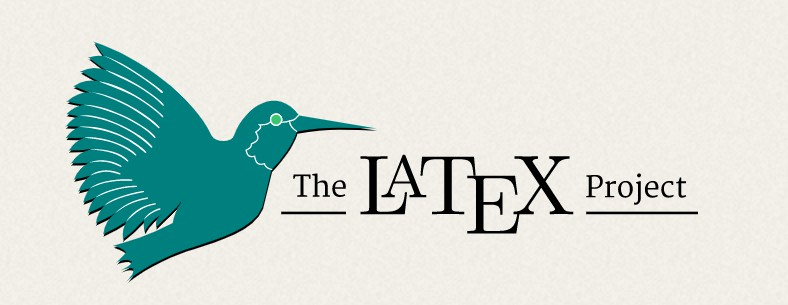
\includegraphics[width=0.7\linewidth]{example.jpg}
    \caption{测试图片}
\end{figure}

\begin{table}[hbt]
    \centering
    \caption{测试表格}
    \begin{tabular}{ c|c|c } 
    \hline
    cell1 & cell2 & cell3 \\
    \hline
    cell4 & cell5 & cell6 \\ 
    \hline
    cell7 & cell8 & cell9 \\ 
    \hline
    \end{tabular}
\end{table}

\begin{equation}
    E=mc^2
\end{equation}

\chapter{标题}
\section{一级节标题}
\subsection{二级节标题}
\subsection{二级节标题}
\subsection{二级节标题}
\section{一级节标题}
\subsection{二级节标题}
\subsection{二级节标题}
\subsection{二级节标题}
\section{本章小结}

\chapter{标题}
\section{一级节标题}
\subsection{二级节标题}
\subsection{二级节标题}
\section{一级节标题}
\subsection{二级节标题}
\subsection{二级节标题}
\section{本章小结}

\makebackmatter

\end{document}